\chapter{Análise Bibliográfica sobre Prova de Conhecimento Zero na Computação, por Gabriel Faustino Lima da Rocha}

\section{Planejamento do estudo}
O pensamento de que para provar a veracidade de uma afirmação é necessário explicar todo o processo que faz a afirmação se tornar verdadeira é comum entre as pessoas, porém uma área da matemática demonstra que isso nem sempre é verdadeiro, através da prova de conhecimento zero.
Por meio desse conhecimento surgiram perguntas sobre os possíveis usos desse campo na computação.

\begin{itemize}
    \item Como a prova de conhecimento zero está sendo utilizada na computação? 
    \item Qual área de pesquisa sofreu maior influencia da prova de conhecimento zero? 
    \item Houve o surgimento de novas áreas devido ao estudo da prova de conhecimento zero?
\end{itemize}

\section{Ferramentas utilizadas}
O pacote Bibliometrix da linguagem R, mais especificamente o biblioshiny, foi utlizado para a criação de dados quantitativos e bibliométricos. O base de dados utlizada foi o Web of Science, WoS, disponível no portal de periódicos da CAPES.

\section{Limitações}
O projeto foi feito ao longo de 3 dias utilizando cerca de 2 horas de cada dia para seu desenvolvimento, o conhecimento prévio do autor sobre as ferramentas e o assunto trado eram superficiais no inicio do projeto.

\section{Coleta de dados}
A coleta de dados foi feita utilizando o WoS no dia 9 de  fevereiro de 2022, por meio do portal de periódicos da CAPES.

As buscas foram reazlidas nas coleções \textbf{Science  Citation  Index  Expanded (SCI -EXPANDED)} e \textbf{Social  Sciences  Citation  Index (SSCI)}.

\subsection{Query de Busca}
A seguinte querry de busca foi utilizada:
\textit{\textbf{zero and knowledge and (proof or protocol}}
Os termos proof e protocol foram utilizados como tendo o mesmo significado, pois a prova de conhecimento zero também pode ser chamada de protocolo de conhecimento zero.

\subsection{Registros recuperados}

Os 1164 registros obtidos como resultado da busca encontram-se em \url{https://github.com/jhcf/Comput-Experim-20212/tree/main/experiments/Faustino27/AnaliseBibliográfica/ZeroKnowledgeProof/TXT}.

Foram utilizadas as opções \textit{Exportar registros para arquivo de texto sem formatação} Seleção personalizada, com todos os 29 campos disponíveis.Os 1164 registros foram exportados em dois blocos, um contendo os registros de 1 até 1000 e o outro o de 1001 até 1164.

\section{Análise dos dados}

\subsection{Filtragem de registros}

Antes da análise foram aplicados filtros nos registros obtidos. Os 1164 registros, após terem o filtro aplicado para apenas publicações em revistas cientificas, resultaram em 870 registros no \dataset nomeado de ZeroKnowledgeProof/Artigos ou ZKPA@Faustino27.

\subsection{Análise descritiva do \dataset\   ZKPA@Faustino27}

As informações principais do \dataset\ ZKPA@Faustino27 são:
\begin{description}
    \item [\textit{Timespan}] Foram encontrado artigos de 1987, até 2021. Não foram encontrados registros entre 1945 e 1986.
    \item [\textit{Sources (Journals, Books, etc)}] São 327 fontes de informação que publicaram os documentos recuperados.
    \item [\textit{Average years from publication}] A média do tempo de publicação dos artigos é de 9,75 anos.
    \item [\textit{Average citations per documents}] Cada artigo foi citado, em média 16,4 vezes.
    \item [\textit{Average citations per year per doc}] Após publicado, cada um dos 870 artigos foi citado, em média, 1,654 vezes por ano.
    \item [\textit{References}] O \dataset\ ZKPA@Faustino27 contém 21.157 referências citadas.
    \item [\textit{Authors}] 2.169 distintos nomes de autores foram encontrados..
    \item [\textit{Authors of single-authored documents}] Dentre os 2.169 distintos (nomes de) autores encontrados, 94 deles editaram artigos individualmente, isso é, sem co-autores.
\end{description}

\subsection{Evolução da Produção Científica}

\begin{figure}
    \centering
    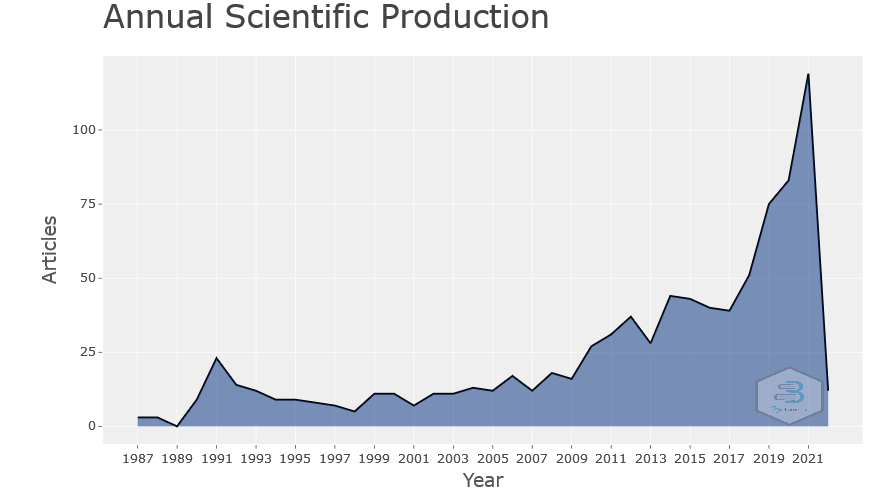
\includegraphics[width=1\textwidth]{experiments/Faustino27/AnaliseBibliográfica/ZeroKnowledgeProof/Imagens/AnnualProduction.png}
    \caption{Evolução da produção científica no \dataset\   ZKPA@Faustino27.}
    \label{fig:evol:anual:ZKPA@Faustino27}
\end{figure}

A figura \ref{fig:evol:anual:ZKPA@Faustino27} mostra a quantidade de artigos publicados sobre o tema escolhido anualmente, é possível observar uma constante quantidade de artigos publicados anualmente até o ano de 2009, depois há um crescimento polinomial até o ano de 2021 em que ocorre uma queda, em 2022 ocorre uma queda, mas provavelmente devido aos dados serem do inicio de fevereiro de 2022, sendo assim não houve tempo para demais artigos serem publicados.

O grande aumento no número de pesquisas recentes mostra o crescimento de interesse sobre o tema no mundo contemporâneo, as pesquisas que incentivaram esse aumento e as áreas que estão crescendo devido a isso serão relatadas mais a frente.

\subsection{Evolução das Citações}

\begin{figure}
    \centering
    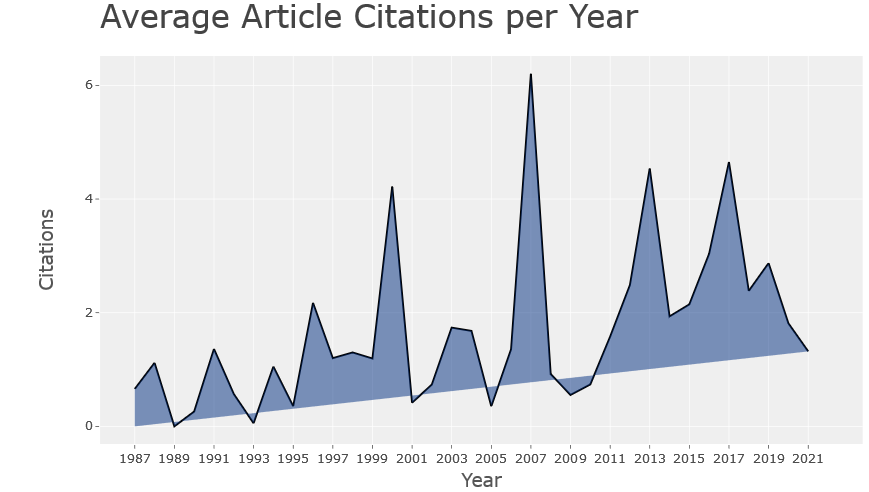
\includegraphics[width=1\textwidth]{experiments/Faustino27/AnaliseBibliográfica/ZeroKnowledgeProof/Imagens/AvarageCitationsYear.png}
    \caption{Evolução das citações ao \dataset\   MASSA@jhcf.}
    \label{fig:evol:anual:citacoes:ZKPA@Faustino27}
\end{figure}

Pelo gráfico \ref{fig:evol:anual:citacoes:ZKPA@Faustino} é possível observar um crescimento na média de citações aos artigos ao passar do tempo, tendo diversos picos, sendo o maior deles em 2007, possivelmente devido a artigos que revolucionaram a área de alguma forma nesses períodos ou a devido ao envolvimento de alguma área nova envolvendo Prova de conhecimento zero.

\subsection{\textit{Three-Field Plots (Sankey diagram)}}

\begin{figure}
    \centering
    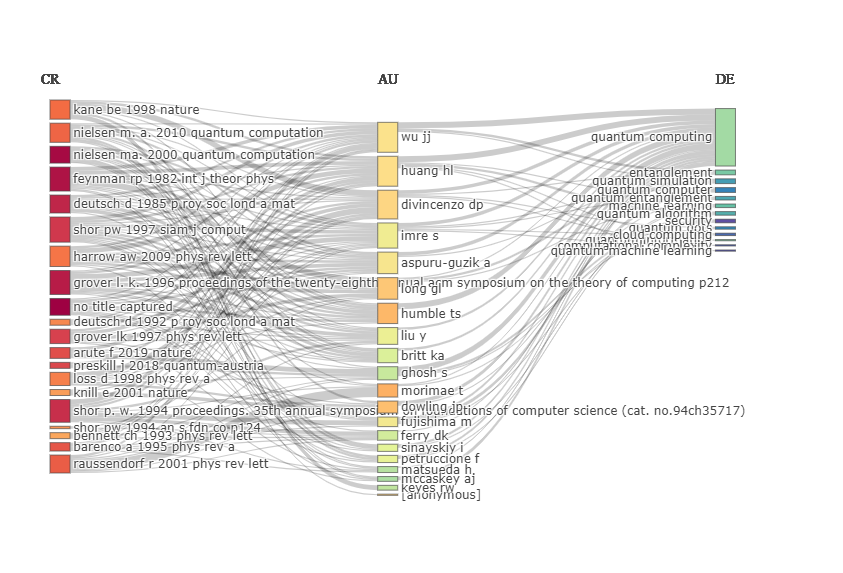
\includegraphics[angle=0,width=1\textwidth]{experiments/Faustino27/AnaliseBibliográfica/ZeroKnowledgeProof/Imagens/ThreeFieldsPlot.png}
    \caption{Plotagem ``Três Campos'' (Sankey plot) do \dataset\   ZKPA@Faustino27: 20 Autores, 20 Citações e 18 Palavras-Chave mais proeminentes.}
    \label{fig:ZKPA@Faustino27:ThreeFieldPlot}
\end{figure}

A figura \ref{fig:ZKPA@Faustino27:ThreeFieldPlot} apresenta a plotagem do tipo ``Três Campos'' do \dataset\  ZKPA@Faustino27, vinculando, ao centro, os 20 Autores mais proeminentes (AU), à esquerda, as 18 Citações mais frequentes (CR - Cited Records), e à direita, as 20 Palavras-Chave mais frequentes empregadas pelos autores.

Podemos observar que os artigos mais citados são os feitos pelo autor Goldwasser S. ocupando a primeira e terceira posição e algumas mais abaixo. O autor Goldreich O. também teve alguns de seus artigos citados, possivelmente por serem os pioneiros na área, no caso de Goldreich O. é possível que seja devido ao seu grande número de artigos publicados.

As palavras chaves mais relacionadas ao tema, tirando o próprio nome do tema, são criptografia, prova interativa e autenticação.Podemos observar que dois desses temas estão relacionados a áreas da computação. Utilizando das demais palavras chaves, vem o tema de encriptação, privacidade, voto eletrônico, algorítimos, e assinatura digital, todos esses voltados a área de computação